%!TEX ROOT=../../Diplomka.tex

\chapter{Implementace}

\section{SPM Motol toolbox}
Vzhledem k faktu, že pro úspěšnou aplikaci výpočtu inverzní úlohy je potřeba provést velké množství přípravných procedur, které jsem naimplementoval do různých funkcí, řešil jsem otázku, jak dostat balík těchto funkcí k lidem, kteří budou metody využívat. Rozhodl jsem se vytvořit SPM Motol toolbox, který obsahuje SPM12 toolbox, upravuje některé jeho funkce a přikládá mnou implementované funkce. Jedná se tedy o rozšíření SPM12 toolboxu. Mezi podstatnou úpravu původního SPM12 toolboxu patří možnost generovat výsledky inverzní úlohy do MRI snímků našich pacientů, namísto do standardního MNI mozku. Přiložené funkce a jejich možnosti si projdeme v~následujících kapitolách.


\subsection{Instalace}
Pro snadné vložení SPM Motol toolboxu do prostředí Matlabu jsem vytvořil \textbf{SPM12Motol\_Installer.m}. Jedná se o instalační skript pro operační systém Windows, který stačí spustit v prostředí Matlab a provede automatické zkopírování toolboxu do složky s ostatními toolboxy a přidá potřebné cesty, díky kterým bude Matlab moci využívat funkce toolboxu v dalších skriptech.

Úspěšnost dokončení instalace lze ověřit pomocí příkazu \textbf{testing\_motol}. Pokud tento příkaz nevypíše chybovou hlášku, je toolbox nainstalován úspěšně.



\section{Předzpracování dat}
Techniky předzpracování dat, neboli preprocessing, jsou procedury nad daty, které připravují data pro další kroky zpracování. Upravují data pro jednodušší nebo efektivnější aplikaci dalších procedur. Nevhodné nebo nedostatečné předzpracování by mohlo vést k zavádějícím výsledkům.

\subsection{Notch filtr}
Notch filtr je filtr typu pásmová zádrž, který se používá k odfiltrování velmi úzké části frekvenčního pásma. Typicky jsou jím filtrovány rušivé signály naindukované na vodiče, které se vždy nacházejí na konkrétním úzkém pásmu frekvence a ovlivňují měření. V podmínkách České republiky jde hlavně o~síťové rušení na kmitočtu 50 Hz (v Americe by se jednalo o 60 Hz).

Skalpové EEG signály jsou velmi slabá napětí v rozsahu od 2 do 200~$\mu$V a~typicky jsou měřena za přítomnosti síťového rušení. Ačkoli je možné zavést opatření, která sníží hladinu síťového rušení, jeho indukci nelze nezabránít úplně. Síťové rušení se může na některých elektrodách projevovat znatelněji než na jiných. Odfiltrování frekvence síťového rušení je tedy nutností. \cite{63}

Pro návrh notch filtru jsem využil membránového konceptu, ze kterého vyplývá, kde musí být umístěny nuly (kořeny čitatele přenosové funkce) filtru v modulu přenosové funkce v z-rovině. První nula musí být umístěna na jednotkové kružnici pod takovým úhlem, který odpovídá frekvenci, kterou chceme odstranit. Druhá nula je poté komplexně sdružená s první. První pól (kořen jmenovatele přenosové funkce) leží v jednotkové kružnici pod stejným úhlem jako první nula. Vzdálenost pólu a příslušné nuly ovlivňuje šířku frekvenčního pásma, které bude filtrem odstraněno. Argument, ovlivňující tuto šířku, bude součástí navrhované funkce. Druhý pól je opět komplexně sdružený prvnímu pólu. \cite{64}

Navrhl jsem Matlab funkci \textbf{Notch}, jejímž vstupem jsou tři argumenty: vzorkovací frekvence, pro kterou filtr navrhujme, frekvence, kterou chceme odstranit a~parametr B, ovlivňující šířku pásma. Výstupem funkce jsou koeficienty čitatele a jmenovatele přenosové funkce filtru.
\begin{figure}[!h]
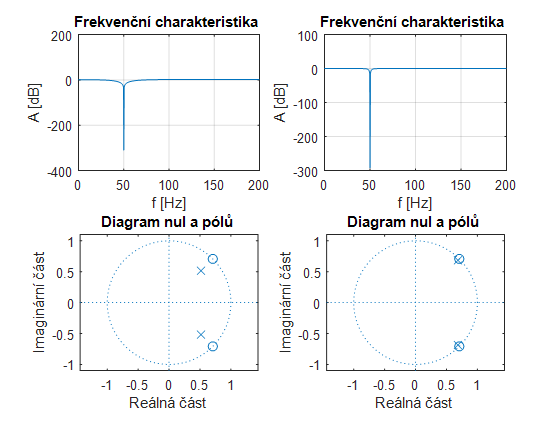
\includegraphics[width=1.0\textwidth]{casti/implementace/notch/charakteristika.png}
\caption{Charakteristiky notch filtrů 50 Hz}
\end{figure}

\newpage
Filtry byly navrženy pro vzorkovací frekvenci 400 Hz, levý sloupec je vykreslen pro šířku pásma 20 Hz, pravý sloupec je vykreslen pro šířku pásma 2 Hz.

\begin{figure}[!h]
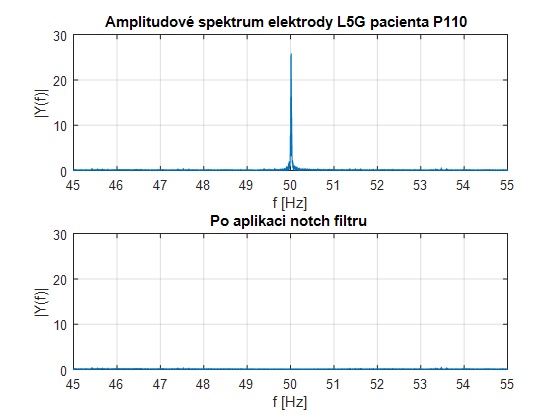
\includegraphics[width=1.0\textwidth]{casti/implementace/notch/aplikace.png}
\caption{Frekvenční spektra reálného EEG signálu před a po aplikaci filtrace notch filtrem}
\label{aplikacedrift}
\end{figure}

V obrázku \ref{aplikacedrift} byl použit notch filtr, navržený pro vzorkovací frekvenci 2048~Hz, zádrž 50~Hz, šířka pásma 1~Hz.

Pro jednoduchou aplikaci jsem připravil funkci \textbf{ApplyNotch}, která automaticky aplikuje filtraci na celý datový soubor. Vstupními argumenty jsou matice dat, jejich vzorkovací frekvence a frekvence, která bude odfiltrována.


\subsection{Odstranění izolinie}
Kolísání izolinie neboli drift je jev, zkreslující naměřená data a objevující se nejen u EEG, ale i u dalších signálů, které je možné na pacientech měřit. Protože se spektra driftu a užitečného signálu překrývají, snažíme se najít takovou metodu, která spektrum užitečného signálu ovlivní nejméně. Kolísání izolinie je způsobeno elektrochemickými ději na rozhraní kůže a elektrody, které jsou následkem nedokonalého kontaktu elektrody a pohyby pacienta. Rušení má náhodný charakter a pro jeho odstranění se používá horní propusť s mezní frekvencí 0,5 Hz. \cite{65,66}

Literatura doporučuje odstranění izolinie pomocí 0,5 Hz hornofrekvenční propusti, při vzorkovací frekvenci 2048 Hz, kterou jsou naměřena EEG data v nemocnici Motol, takový filtr dosahuje nepraktického množství koeficientů. Za použití funkce fir1 pro návrh filtru, přechodové pásmo 0,35 až 0,65 Hz, potlačení 0 dB v propustné části a -40 dB v nepropustné části, dosahuje filtr délky 15 241 koeficientů. Velké množství dat v kombinaci s využitím filtrační funkce filtfilt (filtruje signál dvakrát, od začátku do konce a poté od konce k~začátku, čímž dosahuje nulového zpoždění v signálu), jsou výpočetní nároky příliš vysoké. Pro snížení délky filtru se nabízí možnost decimace signálu, ta ale vyžaduje odstranění aliasing efektu dolní propustí. Pokud bych po odstranění izolinie signál opět interpoloval na původní kmitočet, výsledkem by byl pozměněný signál.

Rozhodl jsem se tedy provést odstranění izolinie jejím odhadem pomocí 0,5 Hz dolní propusti a následným odečtením izolinie od původních dat. Rozdílem od původního přístupu je možnost decimace signálu, aniž bych ovlivnil výsledné spektrum užitečného signálu, čímž dosáhnu kratšího filtru. Signál decimuji faktorem 100, operaci jsem rozložil do dvou decimací faktory 10. Vyšší frekvence, které by mohly být zkresleny aliasingem, budou odfiltrovány aplikací 0,5 Hz dolní propustí. Pro návrh tohoto filtru jsem použil funkce fir1, s přechodovým pásmem 0,35 až 0,65 Hz, potlačením 0 dB v propustné části a -40 dB v nepropustné části. Výsledný filtr má nyní délku pouhých 154 koeficientů a filtrace stejných dat funkcí filtfilt se oproti původnímu přístupu zrychlila cca 75-krát (může se mírně různit v závislosti na vytížení počítače). Aplikací filtrace získám odhad driftu, který lineárně interpoluji na původní frekvenci a odečtu od původních dat.

Celý proces jsem naimplementoval do Matlab funkce \textbf{deleteDrift}. Vstupem funkce je matice s naměřenými EEG daty a vzorkovací frekvence, výstupem jsou EEG data s odstraněným driftem.

\begin{figure}[!h]
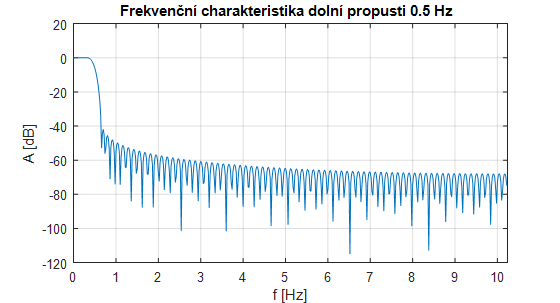
\includegraphics[width=1.0\textwidth]{casti/implementace/izolinie/charakteristika.png}
\caption{Frekvenční charakteristika dolní propusti o mezní frekvenci 0,5 Hz navržená funkcí fir1}
\end{figure}

\begin{figure}[!h]
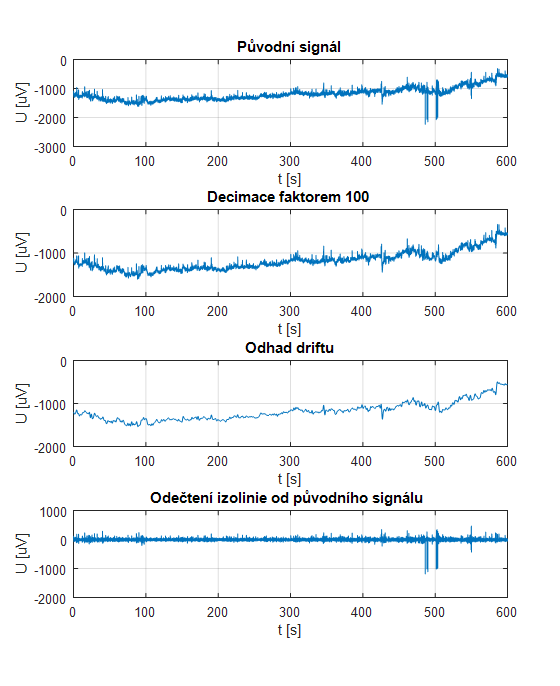
\includegraphics[width=1.0\textwidth]{casti/implementace/izolinie/aplikace.png}
\caption{Proces odstranění izolinie z dat}
\end{figure}

\subsection{Oprava zesilovačů}
Data, naměřená v nemocnici Motol, jsou měřena pomocí sytému firmy ANT Neuro, dnes již nedostupným modelem Asa lab. Tento systém je sice 256-kanálový, ale je složen ze dvou zesilovačů, přičemž každému z nich náleží 128 elektrod. Oba zesilovače měří v referenčním zapojení s průměrnou referencí. U některých pacientů se stalo, že se jednotlivé reference výrazně lišily a hodnoty na elektrodách jednoho zesilovače několikanásobně převyšovaly hodnoty zesilovače druhého. V takovém případě pak inverzní úloha dává nesmyslné výsledky, protože aktivita se nutně objeví pod pozicemi elektrod s vysokými hodnotami.

\begin{figure}[!h]
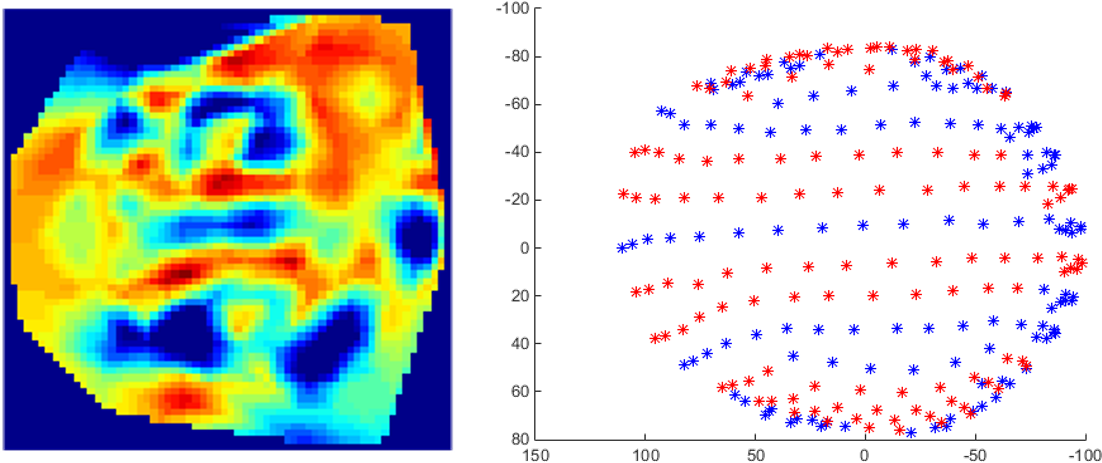
\includegraphics[width=1.0\textwidth]{casti/implementace/opravazesilovacu.png}
\caption{Potenciálová mapa skalpu pacienta, elektrody na skalpu pacienta}
\label{opravazesilovacu}
\end{figure}

Na obrázku \ref{opravazesilovacu} je vidět, že pod modrými elektrodami se vyskytují potenciály s nízkými hodnotami. Červená a modrá barva odlišuje, kterému zesilovači elektroda přísluší.

Tento problém jsme vyřešili přereferencováním signálů obou zesilovačů. V~praxi to znamená, že z každého časového vzorku signálů elektrod jednoho zesilovače je vypočtena průměrná hodnota, která je následně odečtena od hodnot těchto kanálů v tomto časovém vzorku. Stejný postup je aplikován pro signály elektrod druhého zesilovače. Postup se opakuje pro všechny časové vzorky signálu.

Tento proces je naimplementován ve funkci \textbf{amplifierCorrection}, jejímž vstupem je matice dat a dva vektory, ve kterých se nacházejí indexy elektrod jednotlivých zesilovačů. Z těch je následně vypočítána nová reference.



\section{Pomocné funkce}
Kromě funkcí pro předzpracování dat jsem naimplementoval další funkce, které by se v budoucnosti mohly hodit obsluze inverzní úlohy.

\paragraph{Vykreslení pozic elektrod}
Vytvořil jsem funkci \textbf{plotHead}, jejímž vstupem jsou dva argumenty: cesta k~elc souboru, obsahující pozice elektrod a headshape bodů a cesta k elc souboru, který obsahuje body fiducials. Funkce vykreslí trojrozměrný otočný graf s pozicemi elektrod.

\begin{figure}[!h]
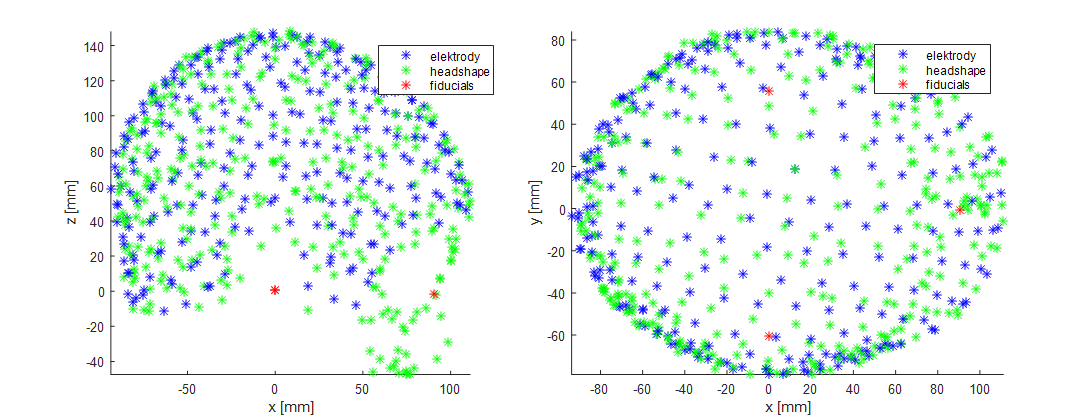
\includegraphics[width=1.0\textwidth]{casti/implementace/head/hlava.png}
\caption{Dvě různá natočení výstupního grafu funkce plotHead}
\end{figure}


\paragraph{Spektrum signálu}
Další užitečnou funkcí je vykreslení jednostranného spektra signálu. Funkce se jmenuje \textbf{signalSpectrum}. Jejím vstupem je cesta k souboru, který obsahuje EEG data, vzorkovací frekvence a vektor s indexy elektrod, jejichž spektrum chceme vykreslit.


\section{Inverzní úloha}
I když pro samotný výpočet inverzní úlohy využívám SPM12 toolbox, stále je potřeba vytvořit potřebné soubory, které budou definovat parametry inverze. Tyto soubory jsou vytvářeny pomocí informací obsažených v datech naměřených na pacientovi. Jejich tvorbu zajišťuje volání jediné funkce.

\subsection{Soubory, potřebné pro výpočet inverzní úlohy}
Prvním ze souborů, potřebných pro výpočet inverzní úlohy, jsou naměřená EEG data. Naměřená data mi jsou předávána v několika souborech Matlab formátu s koncovkou .mat. Rozdělená jsou lépe spravovatelná a umožňují zpracování jen souborů s událostmi, které nás aktuálně zajímají. Každý soubor obsahuje 5 minut EEG záznamů všech elektrod, vzorkovací frekvenci, kterou byla data naměřena, hlavičku, popisující data a vektor, obsahující časy jednotlivých vzorků EEG dat. Hlavička dat je uložena v proměnné header a~obsahuje položky popsané v následující tabulce:

\begin{table}[!h]
\begin{ctucolortab}
\begin{tabular}{lp{8.5cm}}
\bfseries Položka hlavičky & \bfseries Popis \\
\Midrule
header.label & 	Názvy jednotlivých elektrod \\
header.rate & 	Vzorkovací frekvence \\
header.npnt & 	Počet vzorků v datovém souboru \\
header.nchan & 	Počet kanálů datového souboru \\
header.time & 	Vektor časů jednotlivých vzorků EEG dat \\
header.triggers & 	Struktura, popisující události v datech, převážně používaná při měření evokovaných potenciálů \\
header.startdate & 	Datum a čas počátku měření EEG \\
header.triggers\_tabs & 	Časy jednotlivých událostí
\end{tabular}
\end{ctucolortab}
\caption{Popis hlavičky EEG dat}
\label{hlavickaEEG}
\end{table}

K výpočtu inverzního problému dále potřebujeme znát pozice elektrod na skalpu pacienta a pozice bodů fiducials, umožňující správnou koregistraci. Tyto informace jsou zakódovány v souborech s koncovkou .elc a body z nich jsou čteny pomocí funkcí \textbf{elc\_read} a \textbf{fiducials\_read}. Obě funkce mají jeden vstupní parametr, kterým je cesta k příslušnému souboru.

Posledním potřebným souborem je MRI snímek pacientovy hlavy v souboru formátu NIfTI. 

NIfTI (Neuroimaging Informatics Technology Initiative file format) je využíván mnoha softwary zabývajícími se metodami zobrazování, je náhradou za starší ANALYZE formát, který neobsahoval informace o orientaci snímku.
U~NIfTI formátu může také dojít k záměně orientace, uživatel si musí dát pozor, v~jaké rovině software vykresluje snímky.
K záměně levé a pravé strany hlavy může dojít, protože uživatel není schopen určit, ze kterého směru se na řez dívá, zda jde o pohled odspoda nahoru či obráceně. Některé softwary (jako například 3D Slicer) vykreslují snímky v RAS (Right-Anterior-Superior) rovině, kdy se pravá strana hlavy promítne na obrázku vlevo, jiné programy (příkladem je SPM) vykreslují do LPS (Left-Posterior-Superior) roviny.

MRI snímky jsem obvykle obdržel ve formátu Dicom (Digital Imaging and Communications in Medicine). Převedl jsem je na snímky formátu NIfTI pomocí softwaru MRIcron, který je připraven v balíku SPM Motol toolbox spolu s návodem k použití.


\subsection{Načtení EEG dat}
I když je rozdělení EEG dat do více souborů výhodné, pro aplikaci předzpracování je nutné soubory opět spojit do jednoho velkého celku. Pro tento účel jsem vytvořil funkci \textbf{loadEEGData}, jejímž vstupem je cesta ke složce, ve které jsou vybrané soubory pro zpracování uloženy. Metoda postupně načte jednotlivé soubory, jejich data seřadí za sebe a vytvoří jednu společnou hlavičku, popisující data jako celek. Výstup funkce je stejný, jako by byl načten jeden velký soubor s EEG daty.

\subsection{Selekce událostí}
Funkce \textbf{cutTrials}, kterou jsem naimplementoval, umožňuje selekci pouze těch událostí, které nás aktuálně zajímají.
Tato funkce bude použita např. v~případě, kdy se v aktuálně načteném souboru EEG dat somatosenzorických evokovaných potenciálů nacházejí stimulace levé i pravé končetiny. Tato funkce umožní vybrat evokované potenciály pouze jedné z končetin jednoduchým vložením indexů první a poslední události do argumentu funkce.

Funkce \textbf{generateSPMTrialsStruct} vzápětí vygeneruje strukturu, popisující události v datech. Tuto strukturu využijeme v následující funkci.


\subsection{Tvorba souboru kompatibilního s SPM12}
\label{tvorbaSPMsouboru}
Pro analýzu EEG signálu je potřeba převést data do formátu srozumitelného pro SPM12. SPM12 toolbox je schopen automaticky převádět data z různých formátů, jako je biosemi nebo biosig. Využívá k tomu toolboxu fileIO, který je schopen rozpoznat a převést data z většiny komerčních EEG zařízení. Data jsou automaticky převedena do dvou souborů *.dat a *.mat, kde .dat soubor je binární soubor, obsahující EEG záznam a .mat soubor obsahuje hlavičku s~popisem dat a odkazuje se na .dat soubor. Soubory, ve kterých dostáváme data, bohužel nepatří mezi automaticky převeditelné soubory, proto jsem naimplementoval vlastní konvertor. 

Z počátku jsem data převáděl do formátu .gdf. Tento formát je automaticky převoditelný pomocí SPM12 funkce Convert. Od převodu do .gdf jsem ale upustil, protože hlavička souborů tohoto formátu neumožňuje nadefinovat některé potřebné struktury, jako je například struktura popisující události nastalé v datech, nebo struktura popisující pozice elektrod.

Jako další řešení jsem zvolil tvorbu vlastní funkce, která bude převádět data přímo do formátu srozumitelného SPM12. Funkce se jmenuje \textbf{createSPMFile}. Funkce nejprve ověří, zda se shodují názvy elektrod s názvy kanálů v~datech. Pokud není některý kanál nalezen například z důvodu chyby v jeho označení, vypíše se varovná hláška. V dalším kroku je vytvořena proměnná jménem $D$, to je struktura obsahující všechny informace o datech i data samotná. Funkce automaticky vyplní pole hlavičky popsané v tabulkách 
\ref{SPMhlavicka1cast} a \ref{SPMhlavicka2cast}.

\begin{table}
\begin{ctucolortab}
\begin{tabular}{lp{8.5cm}}
\bfseries Položka hlavičky & \bfseries Popis \\
\Midrule
D.type & 	Typ dat: 'continuous', 'single' nebo 'evoked' \\
D.Nsamples & 	Počet vzorků dat \\
D.Fsample & 	Vzorkovací frekvence \\
D.timeOnset & 	Čas prvního vzorku \\
D.data & 	Matice s EEG daty \\
D.fname & 	Jméno souboru, který bude vytvořen \\
D.fpath & 	Cesta k vytvářenému souboru \\
D.trials & 	Celkový popis událostí \\
D.trials.label & 	Názvy nastalých událostí \\
D.trials.onset & 	Čas prvního vzorku první události \\
D.trials.bad & 	Příznak, poukazující na události nevhodné pro další zpracování \\
D.trials.repl & 	V případě průměrovaných dat popisuje, z kolika událostí byla data vytvořena \\
D.trials.events & 	Struktura, popisující události v datech, která byla předpřipravena funkcí generateSPMTrialsStruct \\
D.trials.events.type & 	Název popisované události \\
D.trials.events.value & 	Kódové číslo události \\
D.trials.events.time & 	Čas začátku události v sekundách \\
D.trials.events.duration & 	Doba trvání události \\
D.channels & 	Struktura, popisující kanály záznamu, musí odpovídat pořadí kanálů v datech \\
D.channels.label & 	Název kanálu \\
D.channels.type & 	Typ záznamu - 'MEG', 'EEG', 'VEOG', 'HEOG', 'EMG', 'LFP' \\
D.channels.units & 	Jednotky kanálem měřené veličiny  \\
D.channels.bad & 	Příznak, poukazující na kanál nevhodný pro další zpracování \\
D.channels.X\_plot2D & 	X souřadnice pozice na 2D ploše \\
D.channels.Y\_plot2D & 	Y souřadnice pozice na 2D ploše \\
D.sensors & 	Struktura, upřesňující informace o elektrodách \\
D.sensors.eeg.chanpos & 	Matice, obsahující pozice kanálu na skalpu \\
D.sensors.eeg.chantype & 	Typ záznamu - 'MEG', 'EEG', 'VEOG', 'HEOG', 'EMG' ,'LFP' \\
D.sensors.eeg.chanunit & 	Jednotky kanálů \\
D.sensors.eeg.elecpos & 	Matice, obsahující pozice elektrod na skalpu, totožná s D.sensors.eeg.chanpos \\
D.sensors.eeg.label & 	Názvy kanálů \\
D.sensors.eeg.type & 	Výrobce snímacího zařízení \\
D.sensors.eeg.unit & 	Jednotka souřadnic poloh elektrod
\end{tabular}
\end{ctucolortab}
\caption{Popis hlavičky SPM souboru 1. část}
\label{SPMhlavicka1cast}
\end{table}


\begin{table}
\begin{ctucolortab}
\begin{tabular}{lp{8.5cm}}
\bfseries Položka hlavičky & \bfseries Popis \\
\Midrule
D.fiducials & 	Struktura pro popis tvaru lebky pomocí headshape a fiducials bodů \\
D.fiducials.pnt & 	Matice, obsahující headshape body \\
D.fiducials.fid.pnt & 	Souřadnice tří fiducials bodů \\
D.fiducials.fid.label & 	Názvy těchto fiducials bodů \\
D.history & 	Struktura, uchovávající historii modifikací dat \\
D.history.function & 	Název operace volané na data \\
D.history.arguments & 	Argumenty funkce \\
D.history.time & 	Čas volání funkce \\
D.montage & 	Informace o použitých montážích \\
D.montage.M & 	Transformační matice, popisující operace s kanály a definice nových kanálů, umožňuje například odečítání dvou kanálů pro zisk bipolárního zapojení \\
D.montage.Mind & 	Indikuje, která transformační matice byla použita pro vytvoření dat
\end{tabular}
\end{ctucolortab}
\caption{Popis hlavičky SPM souboru 2. část}
\label{SPMhlavicka2cast}
\end{table}

Takto vytvořená struktura je následně uložena do souboru, který je nyní možné načíst pomocí SPM12 toolboxu a provádět nad ním další operace.

\subsection{Selekce oken a průměrování}
V EEG datech nás typicky zajímají ERP (event related potencials), to jsou malé časové úseky EEG okolo nastalých událostí (takzvaná okna). Proces selekce těchto oken se v SPM12 nazývá epoching. Během tohoto procesu jsou data mimo události odstraněna.

Události jsou jednak reakcí na stimul (evokované potenciály), kdy jsou časy událostí zaznamenány systémem, který vytváří stimuly. Druhou možností jsou události, nastávající náhodně (například komplexy hrot-vlna u epileptiků), jejichž přesné časové umístění dohledáváme pomocí detektorů typických grafoelementů. Ať už se jedná o první nebo druhý typ událostí, okna jsou vždy zatížena náhodnou aktivitou okolních neuronů, která s danou událostí nesouvisí. Proto se vždy snažíme nasbírat co největší množství událostí a~aplikovat metodu průměrování. Vytvořením průměru z oken získáme krátký časový úsek s~nízkou úrovní náhodné aktivity, na který je aplikován výpočet inverzní úlohy. 
Velikost náhodné složky klesá na násobek $\frac{1}{\sqrt{n}}$, kde n je počet realizací.
Náhodná složka by teoreticky byla zcela odstraněna, kdybychom měli k~dispozici nekonečné množství oken.
 
Proces selekce oken a průměrování je již naimplementován v SPM12 toolboxu. Musíme si však připravit pomocný soubor, ve kterém jsou nadefinována okna pro ořez dat. Soubor vytváří funkce s názvem \textbf{prepareTrialsFile}. Vstupem do ní jsou dva argumenty. Je to struktura popisující události, kterou generuje výše popsaná funkce \textbf{generateSPMTrialsStruct} a druhým argumentem je specifikace délky časového okna. Jedná se o vektor dvou časů v~milisekundách, popisující, jak dlouhý časový úsek okolo události bude zachován. Čas událostí je označen nulou, záporný čas označuje dění před událostí. Funkce vygeneruje potřebný soubor a uloží jej do aktuálního adresáře.

Aplikaci selekce oken a průměrování provedeme pomocí Batch editoru SPM12 toolboxu. Jedná se o nástroj, umožňující automatizovat operace nad datovými soubory. Z nabídky funkcí Batch editoru vybereme Preprocessing – Epoching a Averaging. Vstupem epochingu je soubor, obsahující EEG data (výstupní soubor kapitoly \ref{tvorbaSPMsouboru}) a soubor vygenerovaný v minulém kroku, který popisuje, jaká okna budou vybrána. Proces průměrování nastavíme jako závislý, čímž specifikujeme, že průměrování bude aplikováno na výstupní data kroku epoching. Spuštění těchto kroků je možné provést buď přímo v Batch editoru zelenou šipkou v~horní části grafického rozhraní, nebo je možné si vytvořený skript uložit do souboru a kroky spustit pomocí funkce spm\_jobman (soubor je vstupním argumentem), která je součástí SPM12 toolboxu.

\subsection{Výpočet inverzní úlohy}
Specifikaci a výpočet inverzní úlohy je možné v SPM12 toolboxu provést dvěma způsoby. Jedním je využití grafického rozhraní, které je vyvoláno stiskem tlačítka 3D Source Reconstruction. Druhou možností je využitím Batch editoru.

\subsubsection{3D Source Reconstruction}
Uživatelské rozhraní pro výpočet inverzního problému je intuitivní, aktivní jsou vždy jen ta tlačítka, kterými je nutné specifikovat aktuální krok. Výhodou rozhraní je možnost kontroly správnosti jednotlivých kroků, rychlá změna nastavení parametrů inverze a možnost grafického znázornění výsledků inverze v MRI snímcích.

Při prvním spuštění je aktivní pouze tlačítko Load, kterým načteme EEG datový soubor, se kterým budeme pracovat a do kterého se budou jednotlivé kroky ukládat. V druhém kroku specifikujeme model pacientovy hlavy. Máme možnost výběru mezi modelem standardního mozku nebo výpočtem modelu z pacientova MRI snímku. Výpočet modelu trvá několik minut, po dokončení výpočtu se zobrazí vypočtený model hlavy spolu s několika řezy MRI snímkem. Uživatel má tak možnost posoudit, zda byl model vypočten správně (příklad viz \ref{prikladMRImodelu}).

\begin{figure}[!h]
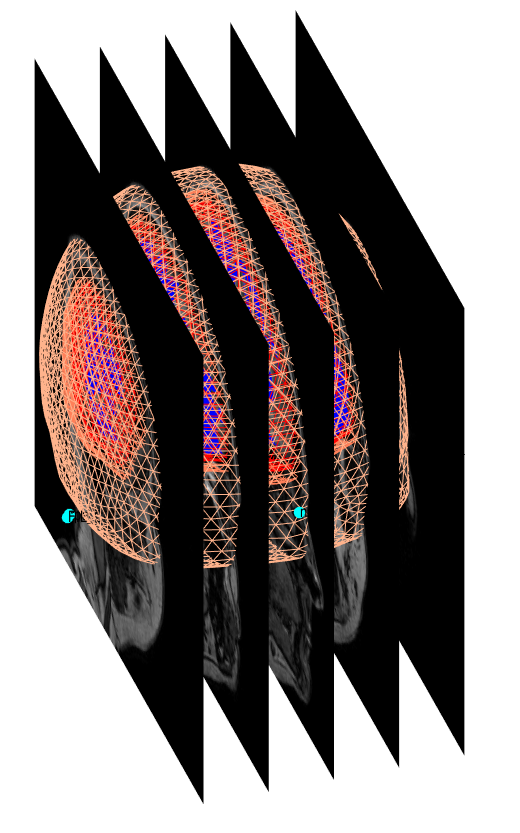
\includegraphics[width = 6cm]{casti/implementace/sourceReconstruction/MRI.png}
\caption{Model vypočtený z MRI snímků pacientovy hlavy}
\label{prikladMRImodelu}
\end{figure}

Následujícím krokem je koregistrace. Rozhraní provede uživatele specifikací bodů fiducials. Ty je možné specifikovat třemi způsoby: výběrem ze seznamu nadefinovaných fiducials, vepsáním souřadnic bodů nebo kliknutím do modelu myší, čímž uživatel určí přibližnou polohu bodů. Po dokončení transformací prostoru MRI a prostoru elektrod je vykreslen výsledek koregistrace, elektrody by měly přesně padnout na skalp modelu (viz \ref{prikladKoregistrace}).

\begin{figure}[!h]
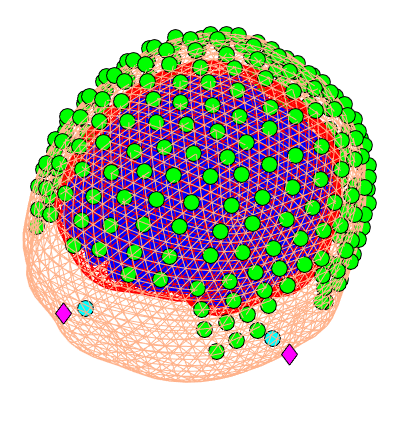
\includegraphics[width = 6cm]{casti/implementace/sourceReconstruction/Corregistration.png}
\caption{Výsledek koregistrace}
\label{prikladKoregistrace}
\end{figure}

Následně je zpřístupněno tlačítko Forward Model, kde dostaneme možnost výběru mezi dostupnými modely. Pro EEG data máme možnost výběru mezi 3-shell sphere nebo BEM modely (modely jsou popsány v kapitole \ref{primaUloha}). Vždy volím anatomicky přesnější a výpočetně náročnější BEM model. Po dokončení finálního výpočtu modelu je model naposledy zobrazen (obrázek viz \ref{3-shell-sphere}). Uživatel provede finální inspekci modelu. Pokud zjistí nesrovnalosti, může kterýkoli z kroků zopakovat a opravit. Dokončením tohoto kroku jsme úspěšně nadefinovali přímou úlohu a v grafickém rozhraní je zpřístupněna možnost výpočtu inverzní úlohy.

Proces výpočtu inverzní úlohy začíná volbou parametrů. Prvním je výběr mezi přeurčenými (tlačítko VB-ECD) nebo nedourčenými modely (tlačítko Imaging). Zvolím nedourčené modely, které jsou intuitivnější a podle mých zkušeností dávají na předložených datech lepší výsledky. Dále máme na výběr mezi dostupnými algoritmy inverzní úlohy (popsány v teoretické části). Následuje možnost volby časového intervalu, na kterém bude algoritmus aplikován a~volba filtru, kterým budou data naposledy filtrována (umožňuje volbu filtraci neprovádět). Poslední možností je zadání apriorní pravděpodobnosti, která specifikuje, ve kterých místech mozku se ložisko nachází s největší pravděpodobností. Takovou informaci ovšem nemáme, pokračujeme tedy bez zadání. Specifikace parametrů inverzní úlohy je tímto kompletní. Výsledek inverze se zobrazí do takzvaného skleněného modelu mozku. Pomocí uživatelského rozhraní máme možnost procházet výsledky inverze pro každý časový vzorek, můžeme spustit film zobrazující vývoj aktivity v čase, nebo výsledky vykreslit do modelu pacientova mozku. Výsledky podporují možnost virtuální elektrody, tedy možnost vykreslení EEG průběhu na zadaných souřadnicích.

\begin{figure}[!h]
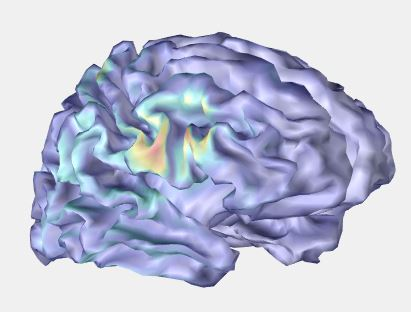
\includegraphics[width=1.0\textwidth]{casti/implementace/sourceReconstruction/render.jpg}
\caption{Příklad výsledku inverzní úlohy, výsledky vykresleny do skleněného mozku a do modelu mozku}
\label{prikladVysledku}
\end{figure}

Pokud není uživatel s výsledkem inverzní úlohy spokojen, může výpočet inverzní úlohy opakovat, použít jiné parametry, zvolit optimální frekvenční pásmo nebo vybrat jiný časový interval. V případě, že je uživatel s výsledky spokojený, může výsledky promítnout přímo do MRI snímků pacientovy hlavy pomocí tlačítka Image.
 
\begin{figure}[!h]
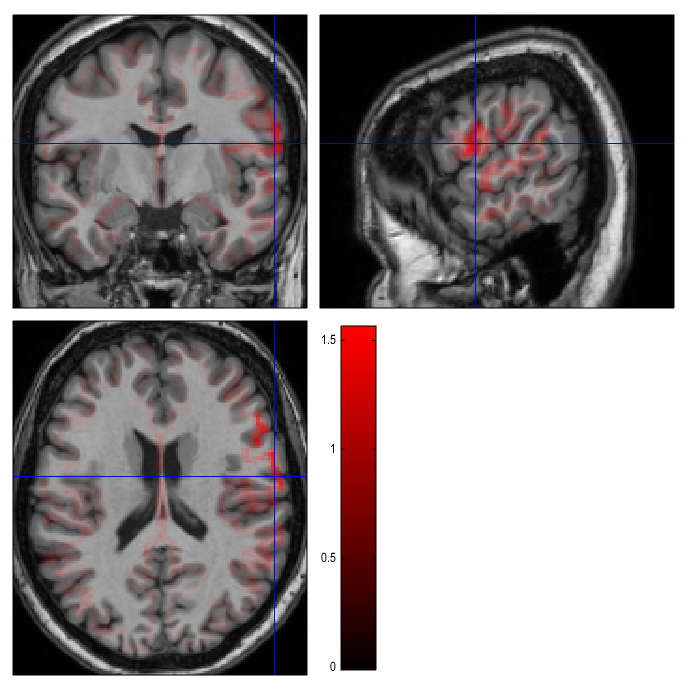
\includegraphics[scale = 0.4]{casti/implementace/sourceReconstruction/vysledek.png}
\caption{Příklad výsledku inverzní úlohy vykresleného do MRI snímku pacienta}
\label{vysledkyMRIsnimek}
\end{figure}

\subsubsection{Batch editor}
Aplikaci inverzní úlohy je možné provést využitím Batch editoru SPM12 toolboxu, provedením operací nazvaných Head model specification a Source inversion. První funkce definuje přímou úlohu, druhá vypočte inverzní úlohu podle zadaných specifikací.

Výhodou tohoto přístupu je možnost automatizace výpočtu, která se hodí v~případech, kdy je nutné zpracovat více případů podobného typu. Nevýhodou je ovšem nemožnost individuálně přistupovat ke každému případu a~kontrolovat správnosti mezikroků. 

Přístup, který jsem shledal nejlepším, je využití kombinace obou, grafického rozhraní i Batch editoru. Automatizuji proces předzpracování dat a~specifikace přímé úlohy pomocí Batch editoru, dále však zpracovávám případ individuálně pomocí grafického rozhraní. Zkontroluji, zda je model hlavy v pořádku, dále vypočítám inverzní úlohu a upravuji její parametry na základě získaných informací. Ve chvíli, kdy jsem s výsledkem spokojen, mohu z~grafického rozhraní pohodlně vykreslit výsledky do MRI snímků. 


\subsubsection{Obalující funkce }
Abych uživatelům SPM Motol toolboxu umožnil jednoduše aplikovat tento postup, naimplementoval jsem obalující funkci jménem \textbf{InversionStart}, jejímž vstupem jsou pouze cesty k EEG a MRI souborům a vstupní proměnné, definující délku okna, které bude použito při epochingu a indexy událostí určených ke zpracování. Díky této funkci je aplikace inverzní úlohy otázkou použití jediné funkce, která se postará o veškeré předzpracování, nadefinuje model pacientovy hlavy, provede koregistraci a vypočte prvotní inverzní úlohu. Uživatel je poté postaven pouze před úkol zlepšovat parametry inverzní úlohy, dokud není spokojený s výsledkem (může například porovnat výsledky metod, zda některá neukáže velmi odlišný výsledek, nebo může upravit uvažované frekvenční pásmo na základě znalosti signálu).

Naimplementoval jsem také podobnou funkci \textbf{InversionStartNoPreprocessing}. Od předcházející funkce se liší pouze tím, že neprovádí předzpracování vstupních dat. Tato funkce je vhodná pro případy, kdy předzpracování provede jiný software, například detektor grafoelementů (jehož výstupem mohou být již zprůměrované grafoelementy hrot-vlna).

